%%%%%%
%
% $Autor: Wings $
% $Datum: 2020-01-18 11:15:45Z $
% $Pfad: TextEnglish.tex $
% $Version: 4620 $
%%%%%%
%
% $Project: AssumptionOfLiability.tex $
% $Version: 4620 $
%
%%%%%%


\begin{tikzpicture}
	\node (Logo) at (0mm,0) {\includegraphics[width=7cm]{Images/Technik}};
	
	
	\node (Adress)  at (10,-22mm) {\begin{tabular}{l} 
			\textbf{\textsf{{\Huge\textcolor{gray}{Der Präsident}}}} \\ 
			\textbf{\textsf{\Large Fachbereich Technik}}\\ 
			\hbox{\vspace{5mm}} \\
			\textbf{\textsf{{\Large\textcolor{gray}{Auskunft erteilt}}}} \\ 
			{\textsf{{Name: Elmar Wings}}}\\ 
			{\textsf{{Name: Elmar.Wings@hs-emden-leer.de}}}\\ 
			{\textsf{{Tel.: 04921 807 1430}}}\\ 
			{\textsf{{Raum: T231}}}\\ 
			
	\end{tabular} };
\end{tikzpicture}	


\vspace{15mm}


\textbf{\textsf{\Large Assumption of Liability}}

\textsf{System \SystemName}

\vspace{15mm}


\StudentName, \StudentNumber:

\bigskip

On \Date, \StudentName{} will take over the following components in perfect condition from the Emden/Leer University of Applied Sciences, MSR Laboratory:

\ListOfMaterials

\StudentName{} is personally liable for the loss of and damage to the components handed over until they are returned.

\vspace{15mm}

Emden, \Date


\vspace{15mm}

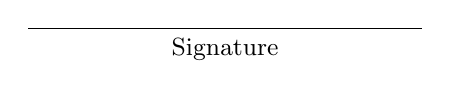
\begin{tikzpicture}
	
	\draw (0,0) -- (50mm,0);
	
	\node[below] (Signature) at (25mm,0) {\small Signature};
	
\end{tikzpicture}	
